Die Funktion
\[
\varphi(x)
=
\begin{cases}
ax^2&\qquad 0\le x\le 1\\
a(x-2)^2&\qquad 1\le x \le 2\\
0&\qquad\text{sonst}
\end{cases}
\]
soll als Wahrscheinlichkeitsdichte einer Zufallsvariablen $X$ verwendet
werden können.

\begin{figure}[ht]
\centering
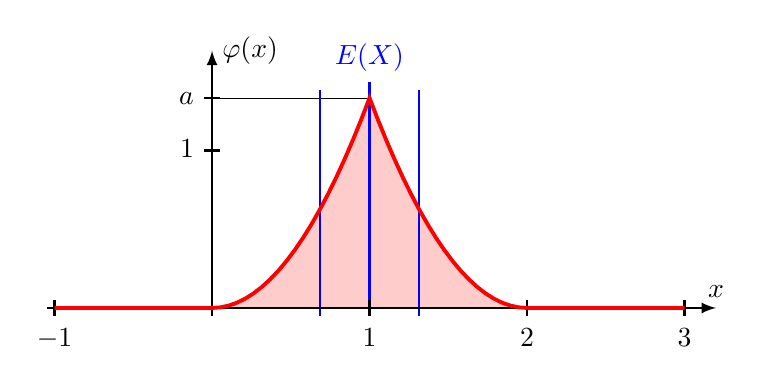
\begin{tikzpicture}[>=latex,thick,scale=2]
\def\a{1.3333}
\pgfmathparse{sqrt(0.1)}
\xdef\varianz{\pgfmathresult}
\draw[line width=0.2pt] (0,\a) -- (1,\a);
\draw (-0.05,\a) -- (0.05,\a);
\node at (-0.05,\a) [left] {$\mathstrut a$};
\fill[color=red!20] 
	plot[domain=0:1,samples=20] (\x,{\a*\x*\x})
	--
	plot[domain=1:2,samples=20] (\x,{\a*(\x-2)*(\x-2)})
	-- cycle;
\ifthenelse{\boolean{loesungen}}{
\draw[color=blue] ({1-\varianz},-0.05) -- ({1-\varianz},{\a+0.05});
\draw[color=blue] ({1+\varianz},-0.05) -- ({1+\varianz},{\a+0.05});
\draw[color=blue] (1,0) -- (1,{\a+0.1});
\node[color=blue] at (1,{\a+0.1}) [above] {$E(X)$};
}{}
\draw[->] (-1.05,0) -- (3.2,0) coordinate[label={$x$}];
\draw[->] (0,-0.05) -- (0,{\a*1+0.3}) coordinate[label={right:$\varphi(x)$}];
\foreach \x in {-1,1,2,3}{
	\draw (\x,-0.05) -- (\x,0.05);
	\node at (\x,-0.05) [below] {$\x\mathstrut$};
}
\draw (-0.05,1) -- (0.05,1);
\node at (-0.05,1) [left] {$\mathstrut 1$};
\draw[color=red,line width=1.4pt] (-1,0) --
	plot[domain=0:1,samples=20] (\x,{\a*\x*\x})
	--
	plot[domain=1:2,samples=20] (\x,{\a*(\x-2)*(\x-2)})
	--
	(3,0);
\end{tikzpicture}
\caption{Graph der Funktion $\varphi(x)$ von Aufgabe~\ref{50000050}
\label{50000050:fig}}
\end{figure}

\begin{teilaufgaben}
\item
Wie muss $a$ gewählt werden?
\item
Bestimmen Sie $E(X)$.
\item
Bestimmen Sie die Varianz $\operatorname{var}(X)$.
\end{teilaufgaben}

\begin{loesung}
Man beachte, dass die Funktion $\varphi(x)$ symmetrisch ist bezüglich $x=1$.
Dies ermöglicht, die Berechnung der Integrale zu vereinfachen.
\begin{teilaufgaben}
\item
$a$ muss so gewählt werden, dass die Normierungsbedingung
\[
\int_{-\infty}^{\infty} \varphi(x)\,dx =1
\]
erfüllt ist.
Wegen der genannten Symmetrie genügt es dazu, dass
\[
\frac12
=
\int_0^1 ax^2\,dx
=
\left[
\frac{ax^3}3
\right]_0^1
=
\frac{a}{3}.
\]
Auflösen nach $a$ ergibt $a=\frac32$.
\item
Da $\varphi(x)$ symmetrisch bezüglich $1$ ist, ist $E(X)=1$.
\item
Die Varianz kann mit Hilfe der Formel $\operatorname{var}(X)=E(X^2)-E(X)^2$
berechnet werden.
\begin{align*}
E(X^2)
&=
\int_{-\infty}^\infty x^2\varphi(x)\,dx
=
\int_0^1 ax^4\,dx
+
\int_1^2 a(x-2)^2x^2\,dx
\\
&=
a\left[\frac{x^5}{5}\right]_0^1
+
a\int_1^2
x^4-4x^3+4x^2\,dx
\\
&=
\frac{a}5
+
a
\left[
\frac{x^5}5
-x^4
+\frac43x^3
\right]_1^2
=
\frac{a}5
+a\biggl(\frac{31}5-15+\frac{28}3\biggr)
=\frac{11a}{15}
=
\frac{11}{10}.
\\
\operatorname{var}(X)
&=
E(X^2) - E(X)^2
=
\frac{11}{10}-1
=
\frac{1}{10}
=
0.1.
\end{align*}
Der Erwartungswert sowie das Interval zwischen
$E(X)-\sqrt{\operatorname{var}(X)}$
und
$E(X)+\sqrt{\operatorname{var}(X)}$
ist in Abbildung~\ref{50000050:fig} blau eingezeichnet.
\qedhere
\end{teilaufgaben}
\end{loesung}

\begin{bewertung}
\begin{teilaufgaben}
\item Normierunbsbedingung ({\bf N}) 1 Punkt, Wert für $a$ ({\bf A}) 1 Punkt.
\item Wert für $E(X)$ ({\bf E}) 1 Punkt.
\item Varianzformel $\operatorname{var}(X)=E(X^2)-E(X^2)$ ({\bf F}) 1 Punkt,
Ansatz für die Berechnung von $E(X^2)$ ({\bf X}) 1 Punkt,
Wert der Varianz ({\bf V}) 1 Punkt.
\end{teilaufgaben}
\end{bewertung}
